\documentclass{beamer}
\usepackage{amsmath}
\usepackage{euler}
\usepackage{graphicx}
\usepackage{subcaption}
\usepackage{hyperref}
\usetheme[progressbar = frametitle]{metropolis}
\setbeamertemplate{frame numbering}[fraction]
\title{Generalised Gradient Approximation}
\author{Elious}
\date{}

\begin{document}
\metroset{block=fill}
	\begin{frame}
	\titlepage
	\end{frame}
	\begin{frame}[t]{Lets recap some LDA}
	\textbf{Assumption} : electron density of inhomogenoues system is locally homogenous.The exchange-correlation energy is thus given by: 
	\begin{equation}\label{eq:1}
	E_{xc}^{LDA} = \displaystyle{\int }\rho(\textbf{r})\epsilon_{xc}^{h}(\rho(\textbf{r}))d\textbf{r}
	\end{equation}
	and 
	\begin{equation}\label{eq:2}
	E_{xc}^{LSDA} = \displaystyle{\int }\rho(\textbf{r})\epsilon_{xc}^{h}(\rho_{\uparrow}(\textbf{r}),\rho_{\downarrow}(\textbf{r}))d\textbf{r}
	\end{equation}
	where
	$\epsilon_{xc}^{h}(\rho(\textbf{r})) \rightarrow$ exchange-correlation energy density at \textbf{r}, evaluated by taking the $E_{xc}$ of the uniform gas with density $\rho(\textbf{r})$
	\end{frame}
	
	\begin{frame}[t]{Intuition for LDA}
	\begin{figure}
	\centering
	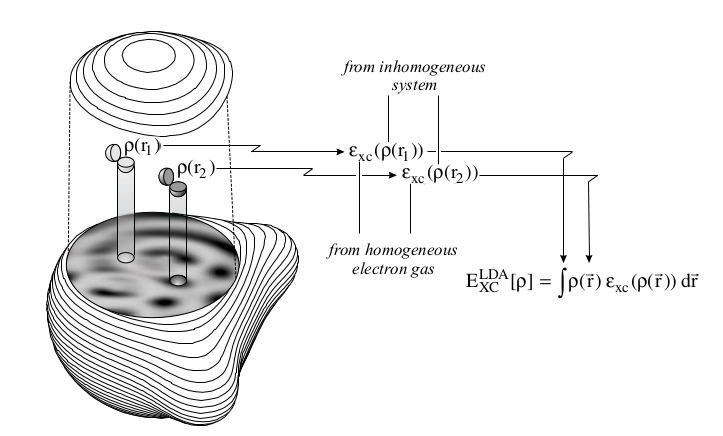
\includegraphics[scale=0.40]{LDA_intuition.png}
	\end{figure}
	Taken from : W.Koch, M.C. Holthausen ,Chemists Guide To DFT
	\end{frame}		
	
	\begin{frame}[t]{Expectations}
	 \begin{columns}
      \begin{column}{0.48\textwidth}
        \begin{figure}[t]
	  	 \begin{subfigure}{1.\textwidth}
  		  
\includegraphics[width=1.\linewidth]{LDA_perfect.jpeg}
 	     \end{subfigure}
 	     \begin{subfigure}{1.\textwidth}
  		  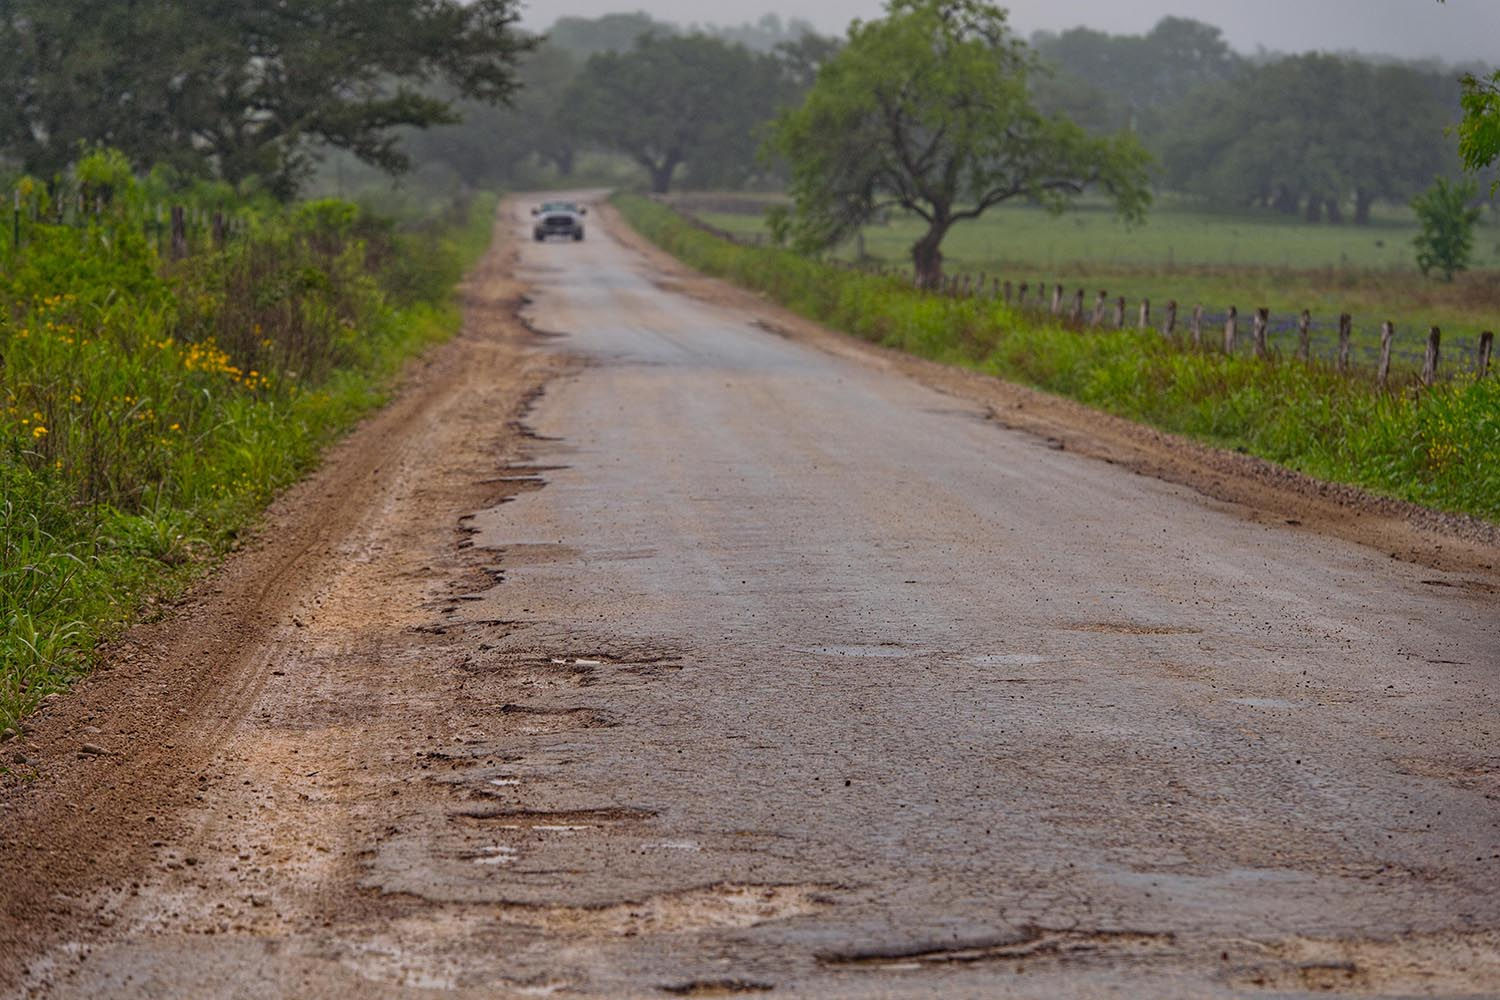
\includegraphics[width=1.\linewidth]{LDA_works.jpeg}  
 	     \end{subfigure}
	     \caption{LDA should work fine}
	    \end{figure}
      \end{column}
      \begin{column}{0.48\textwidth}
        \begin{figure}[t]
	  	 \begin{subfigure}{.9\textwidth}
  		  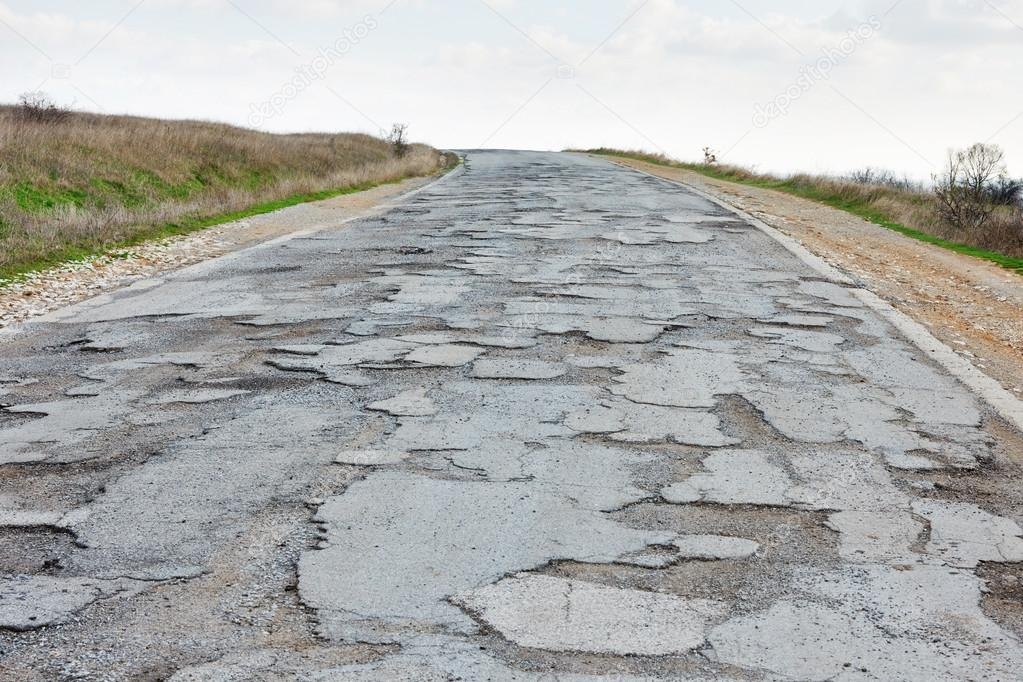
\includegraphics[width=1.\linewidth]{LDA_approx.jpg}
 	     \end{subfigure}
 	     \begin{subfigure}{.9\textwidth}
  		  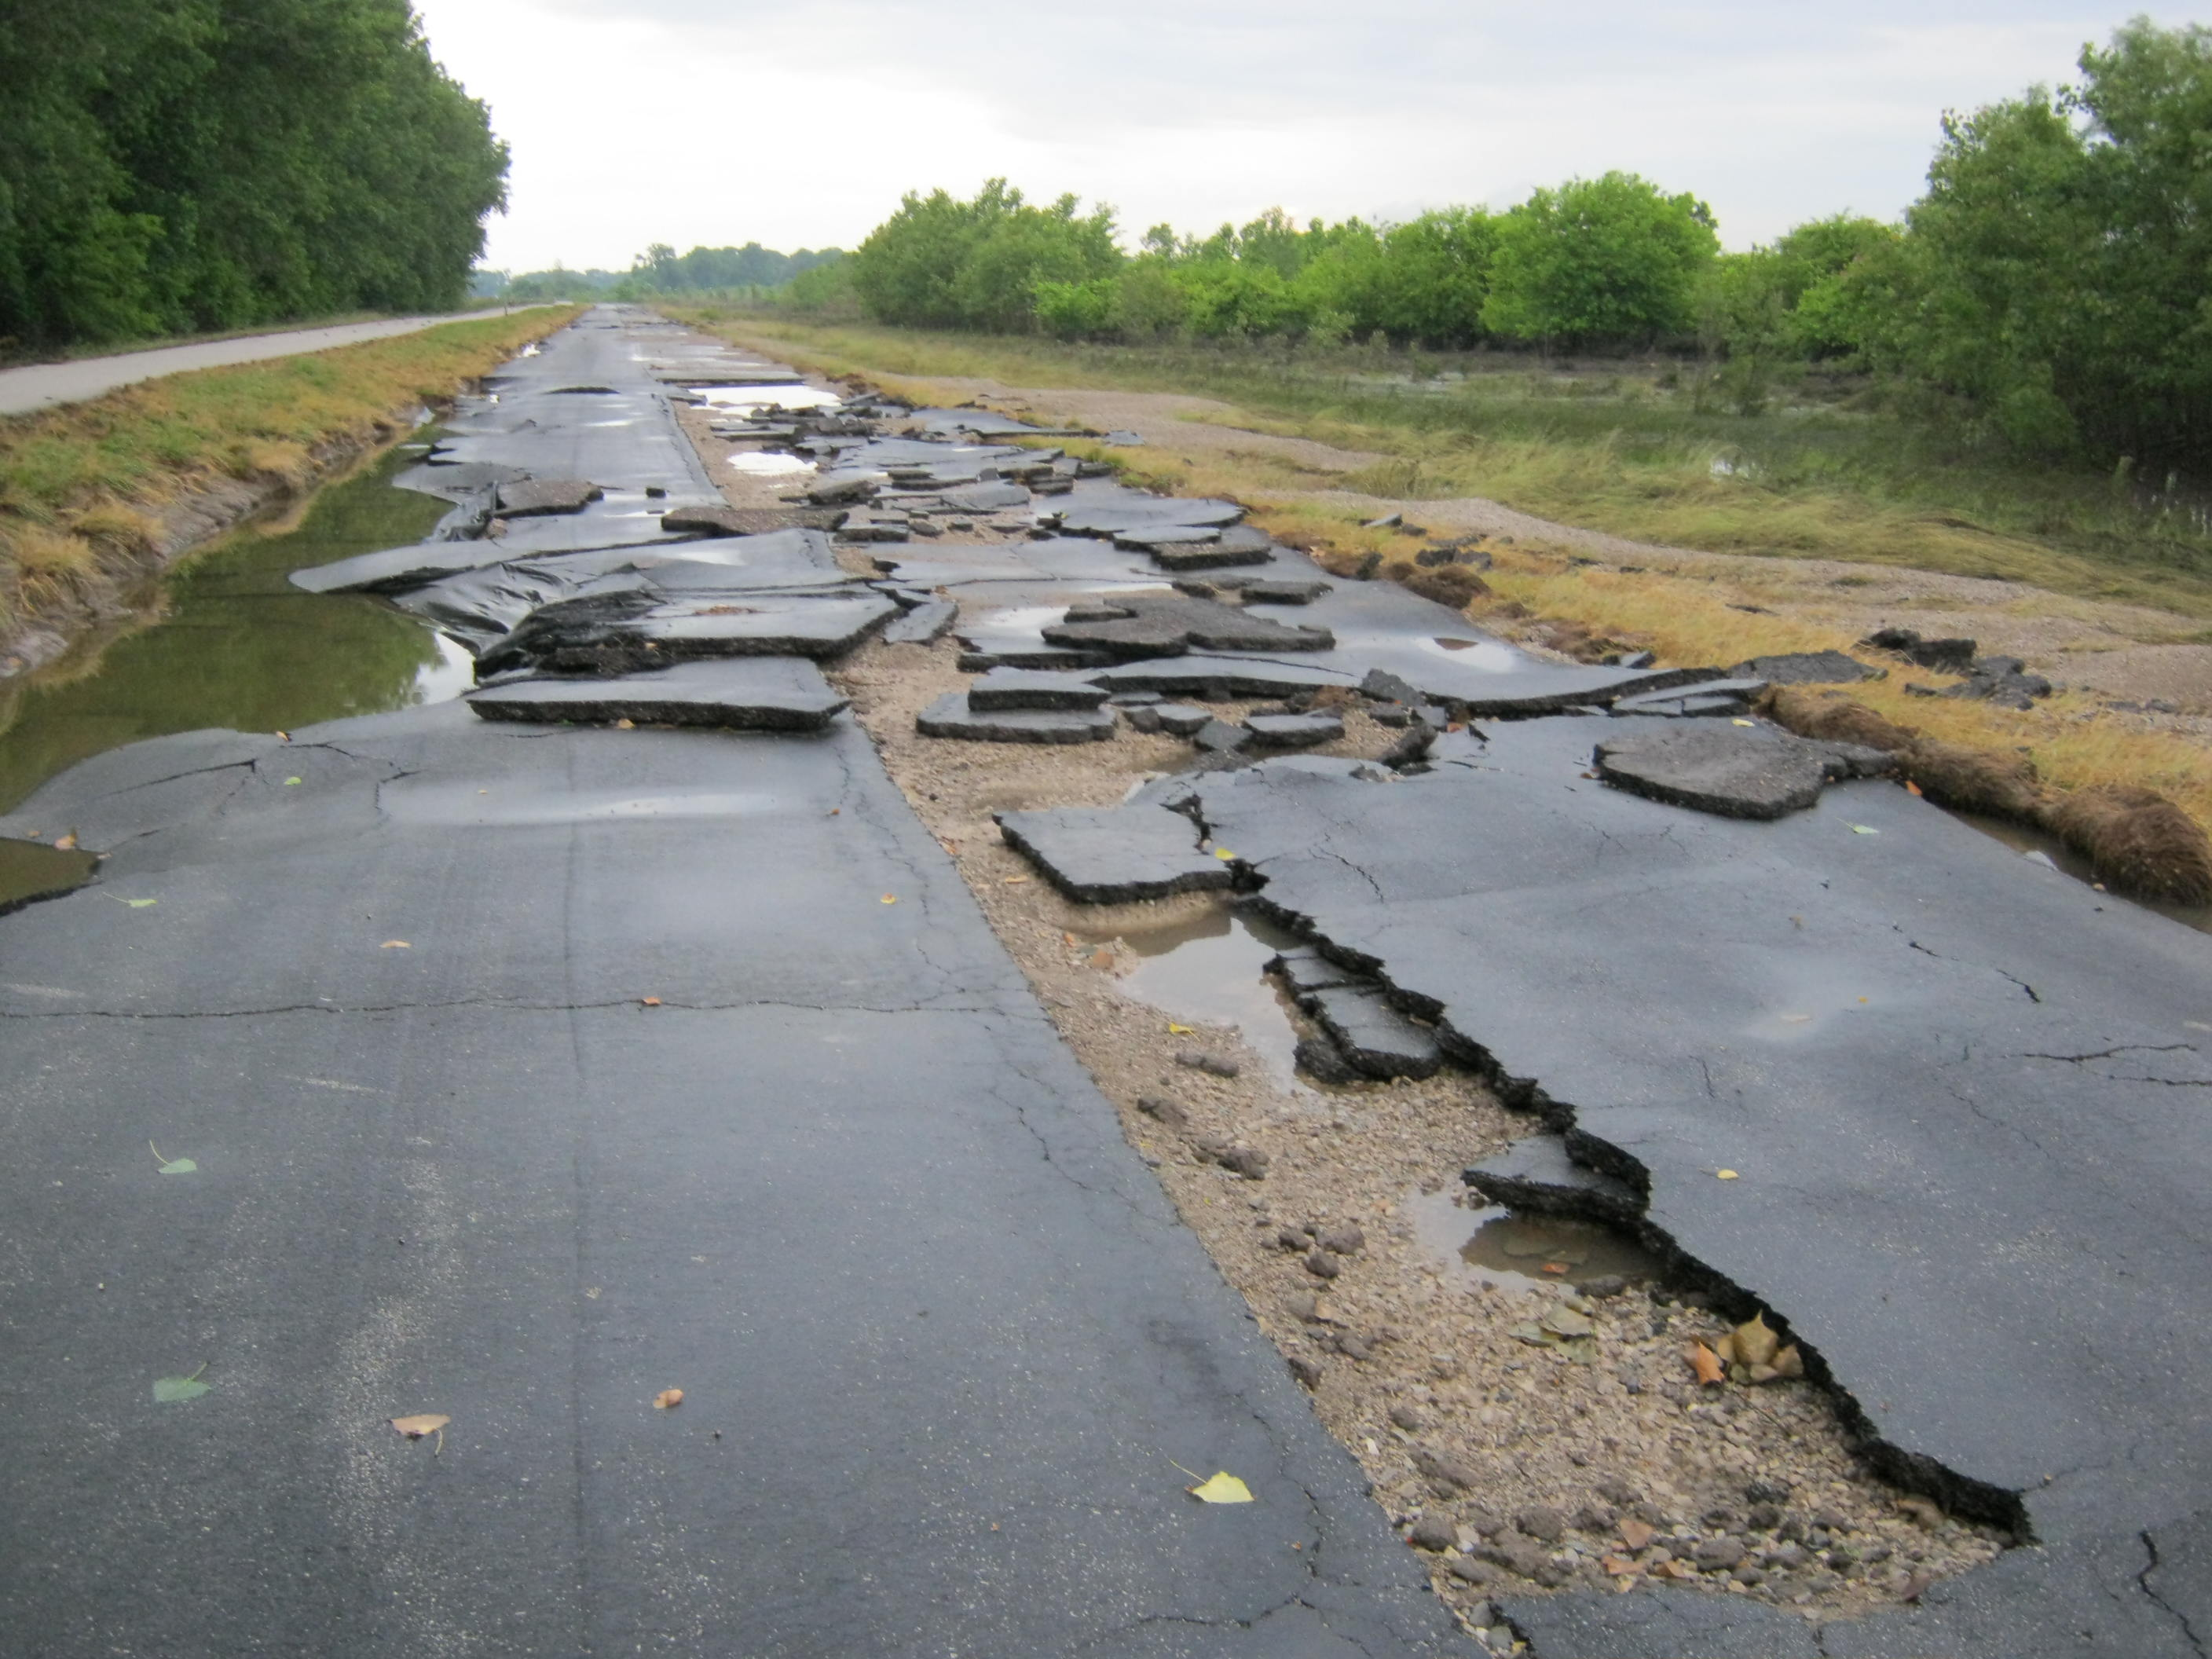
\includegraphics[width=1.\linewidth]{LDA_breaks.jpg}  
 	     \end{subfigure}
	     \caption{LDA should be useless}
	    \end{figure}
      \end{column}
	 \end{columns}
	\end{frame}
	
	\begin{frame}[t]{Reality}
	 \begin{large}
	  \textbf{LDA works considerably well in all the above cases!!!}
	 \end{large}
	 \begin{enumerate}
	   \item{It works nearly perfect for many properties of metals.}
	   \item{It even predicts molecular properties like equilibrium structures, charge moments etc.}
	   \linebreak
	  \end{enumerate}
	  \textbf{However}, the energy details are not so good for the inhomohenous systems.Comparing with the experiments, the unsigned standard deviation:
	  \begin{equation}\label{eq:3}
	  	\Delta_{LDA} = 36 Kcal/mol (1.56 eV)
	  \end{equation}
	  \begin{equation}	\label{eq:4}   
	  	\Delta_{HF} = 78 Kcal/mol (3.38 eV)
	  \end{equation}
	  \large{\textbf{But, Why should the LDA even work at all for the inhomogenous system???}}
	\end{frame}
	
	\begin{frame}[t]{Lets find some holes in LDA}
	 \begin{equation}\label{eq:5}
	 E_{xc}[\rho] = \frac{1}{2}\displaystyle{\int}\displaystyle{\int} \frac{\rho(\textbf{r}_1)\rho_{xc}(\textbf{r}_1;\textbf{r}_2)}{|\textbf{r}_1-\textbf{r}_2|}d\textbf{r}_1 d\textbf{r}_2
	 \end{equation}
	 where\\
	 $\rho(\textbf{r}_1) d\textbf{r}_1 \rightarrow$ Probability density of finding an electron in $d\textbf{r}_1$ near $\textbf{r}_1$\\
	 $\rho_{xc}(\textbf{r}_1;\textbf{r}_2) d\textbf{r}_2 \rightarrow$ Probability density of finding an electron in $d\textbf{r}_2$ near $\textbf{r}_2$ given there is an electron in $d\textbf{r}_1$ near $\textbf{r}_1$. This is called the \textbf{exchange-correlation hole}. We can show\\
	\begin{equation}\label{eq:6}
	 \displaystyle{\int} \rho_{xc}(\textbf{r}_1;\textbf{r}_2) d\textbf{r}_2 = -1
	\end{equation}
	and
	\begin{equation}\label{eq:7}
	\rho_{xc}(\textbf{r}_1;\textbf{r}_2) \leqslant 0
	\end{equation}
	we usually do:
	\begin{equation}\label{eq:8}
	\rho_{xc}(\textbf{r}_1;\textbf{r}_2) = \rho_{x}(\textbf{r}_1,\textbf{r}_2) + \rho_{c}(\textbf{r}_1,\textbf{r}_2)
	\end{equation}
	\end{frame}	
	
	\begin{frame}[t]{Pair-correlation factor}
	The $\rho_{xc}(\textbf{r}_1;\textbf{r}_2)$ is factorised as the product:
	\begin{equation}\label{eq:9}
	\rho_{xc}(\textbf{r}_1;\textbf{r}_2) = \rho(\textbf{r}_2)f_{xc}(\textbf{r}_1;\textbf{r}_2)
	\end{equation}
	here 
	\begin{equation}\label{eq:10}
	-1\leqslant f_{xc}(\textbf{r}_1;\textbf{r}_2) \leqslant 0
	\end{equation}
	Combining eqn(\ref{eq:9} and \ref{eq:10}) we can see that the factorisation is just another way of saying that there is \textbf{reduction of electron density} from $\textbf{r}_2$. The factor $f_{xc}(\textbf{r}_1;\textbf{r}_2)$ is called the pair-correlation factor.\\
	We should note that:
	\begin{enumerate}
	\item{The XC-hole is non-spherical as it depends on $\rho(\textbf{r}_2)$ which is usually non-uniform.}
	\item{For LDA XC-hole is spherical as $\rho(\textbf{r}_2)$ is uniform.}
	\end{enumerate}
	\end{frame}
	
	\begin{frame}[t]{Intuition for XC-hole}
	\begin{figure}
	\centering
	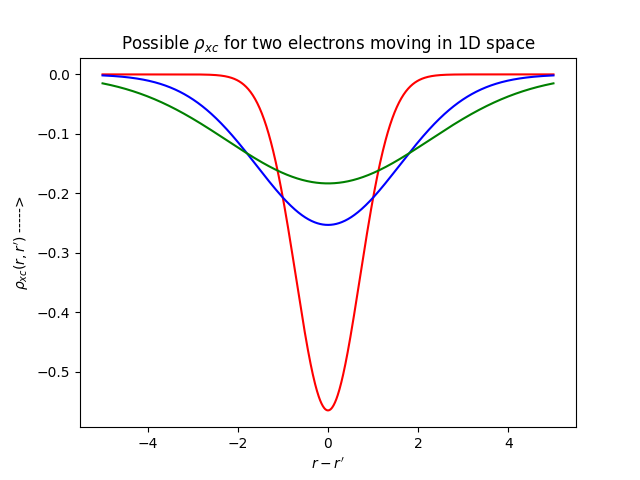
\includegraphics[scale=0.65]{nxc.png}
	\end{figure}
	\end{frame}		
	
	\begin{frame}[t]{Exchange hole}
	\textbf{Exchange (Fermi) hole} : We can show that for the Kohn-sham system $\rho_{xc}(\textbf{r}_1;\textbf{r}_2)$ arises due to \textit{Pauli-repulsion} of same spin electrons and from there 
	\begin{equation}\label{eq:11}
	\rho_{x}(\textbf{r}_1;\textbf{r}_2) \leqslant 0
	\end{equation}
	and
	\begin{equation}\label{eq:12}
	\displaystyle{\int} \rho_{x}(\textbf{r}_1;\textbf{r}_2) d\textbf{r}_2 = -1
	\end{equation}
	\begin{enumerate}
	\item{From eqn(\ref{eq:11}) the hole is negative everywhere $\rightarrow$ an electron of a spin $\sigma$ won't allow another electron of the same spin to occupy its orbital.}
	\item{Also since its negative everywhere $\rightarrow$ it must be responsible for the self-interaction correction.}
	\end{enumerate}
	\end{frame}
	
	\begin{frame}[t]{Correlation Hole}
	We are now left with the \textbf{Correlation (Coulomb) hole} which mainly arises due to $1/r_{ij}$ nature of the coulomb repulsion
	\begin{equation}\label{eq:13}
	\displaystyle{\int} \rho_{c}(\textbf{r}_1;\textbf{r}_2) d\textbf{r}_2 = 0
	\end{equation}
	So  it's positive in some regions and negative in some regions thus integrating out to zero...???\\We can think of this like
	\begin{enumerate}
	\item{Due to $1/r_{ij}$, at the region near any electron, the other electron will be repelled the highest(the hole is negative in this region) and thus it will be sent to a far away region $\rightarrow$ piling up density in other region i.e. the hole is positive in this region.}
	\item{Since this is due to $1/r_{ij}$, $\rho_c$ will also be responsible for the electron-electron cusp in the many-electron wavefunction.}
	\end{enumerate}
	\end{frame}
	
	\begin{frame}[t]{Intuition for X and C-hole}
	\begin{figure}
	\centering
	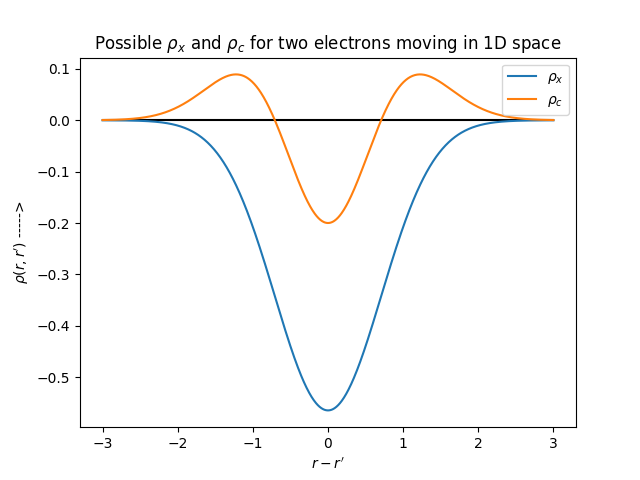
\includegraphics[scale=0.65]{nx_nc.png}
	\end{figure}
	\end{frame}
	
	\begin{frame}[t]{Summary of XC-holes}
	\begin{enumerate}
	\item{\textbf{Exchange hole :} Two electrons of same spin cannot occupy the same room \textit{aka} \textbf{Pauli's exclusion Principle}}\\
	\vspace{0.5cm}
	\item{\textbf{Correlation hole :} Two electrons can live in the same room but they have to follow social-distancing norms.}\\
	\vspace{0.5cm}
	\item{eqn(\ref{eq:5}) shows that $E_{xc}$ is actually the energy of attraction of an electron density with its hole $\rightarrow$ the better our model hole represents the exact hole, the better it will represent the $E_{xc}$}
	\end{enumerate}
	\end{frame}
	
	\begin{frame}[t]{Back to the questions}
	\textbf{Question1:} Why does LDA perform well even for inhomogenous densities?\\
	\textbf{Answer: }LDA is for homogenous electron gas $\rightarrow$nicely represents some of the exact properties of holes defined above:
	\begin{enumerate}
	\item{The sum rules are satisfied}
	%\item{$n_x(\textbf{r}_2\rightarrow\textbf{r}_1;\textbf{r}_1) = -\rho(\textbf{r}_1)$}
	\item{The cusp condition of the correlation is satisfied}
	\item{$n_x(\textbf{r}_2;\textbf{r}_1)\leqslant 0 $ everywhere}
	\end{enumerate}
	\vspace{0.5cm}
	\textbf{Question2:} What is the problem with LDA?\\
	\textbf{Answer: } LDA is for homogenous electron gas$\rightarrow$tends to homogenise the properties for inhomogenous systems.Eg: It leads to overbinding in molecules.
	\end{frame}
	
	\begin{frame}[t]{Overbinding in LDA - A step by step guide}
	\begin{enumerate}
	\item{Atoms have a highly inhomogenous electron density}
	\item{Molecules have a relatively more homogenous electron density compared to atoms as electrons are now more delocalised around two(or more atoms) but still its inhomogenous}
	\item{LDA best approximates homogenous electron density}
	\item{LDA tends to homogenise the electron density more in the molecule}
	\item{More bonding character in molecule than should be present}
	\item{Exchange energy of the molecule is too negative $\rightarrow$ Overbinding}
	\end{enumerate}
	\end{frame}
	
	\begin{frame}[t]{Overbinding in LDA - the process}
	 \begin{figure}
	  \centering
	  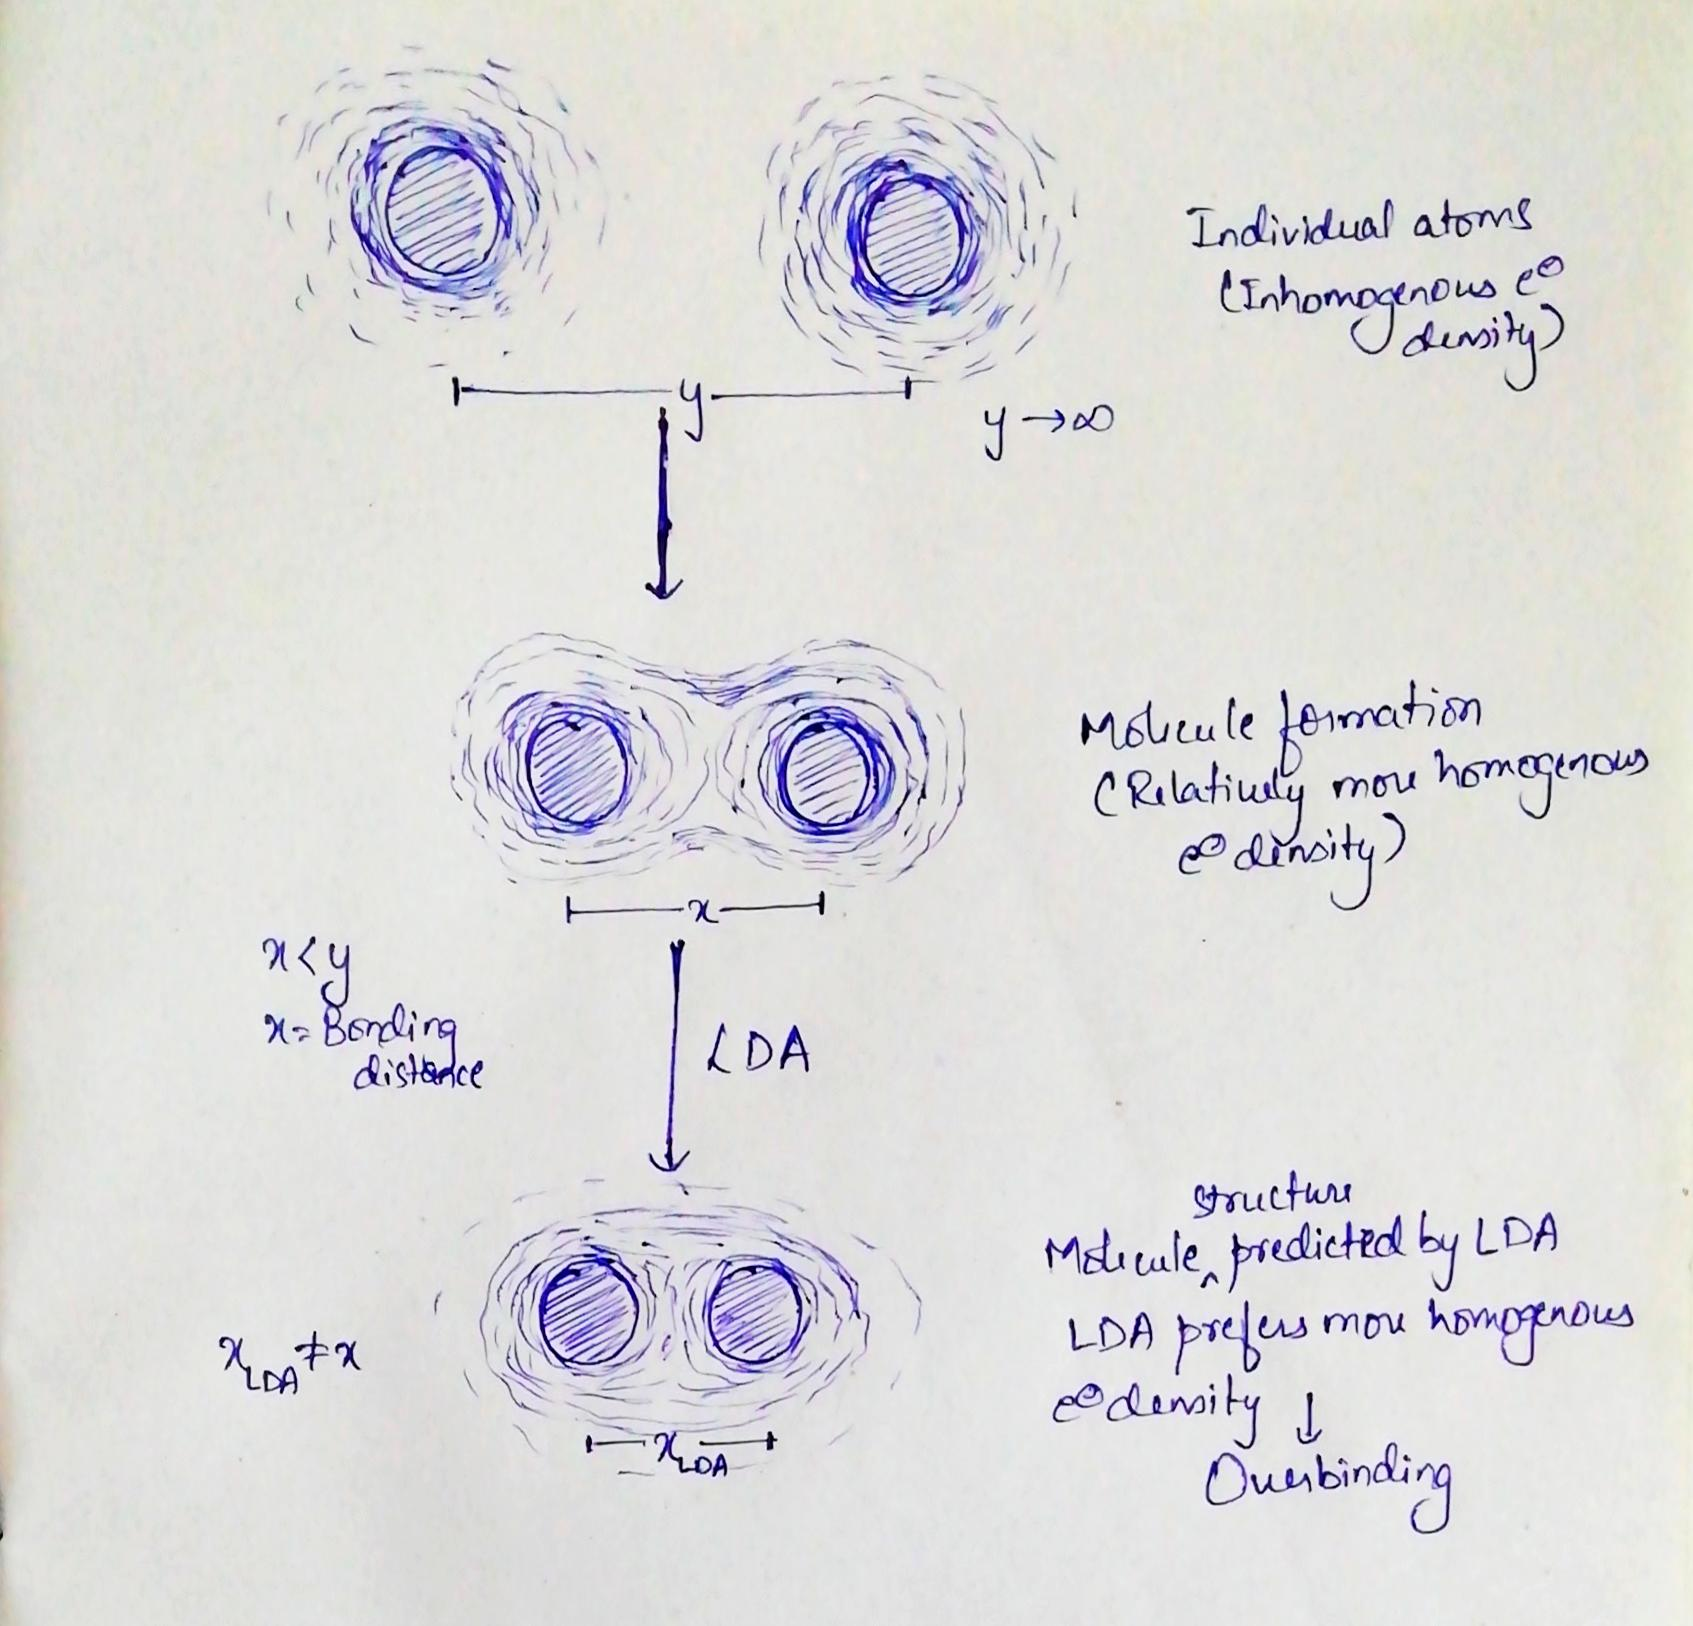
\includegraphics[scale=0.135]{LDA_overbinding.jpg}
	 \end{figure}
	\end{frame}
	
	\begin{frame}[t]{Gradient expansion (Ma and Brueckner, 1968)}
	
	\begin{block}{\textbf{Idea:}}
	\begin{enumerate}
	\item{ Divergence from uniformity of the electron density is due to perturbation to the system}
	\item{Perturb the homogenous system with little distortions in the potential.}
	\item{Attempt a solution by taylor expansion of density around the homogenous electron density}
	\end{enumerate}
	\end{block}
	
	So we can try:
	\begin{equation}\label{eq:14}
		\rho^{inh}(\textbf{r}) \rightarrow \rho^{h}(\textbf{r})\left[1+\nabla \rho^h(\textbf{r'})|_{\textbf{r'=r}} + \mathcal{O}(\nabla^2 \rho^h(\textbf{r})) \right]
	\end{equation}
	and what's done in GE is: 
	\begin{equation}\label{eq:15}
	 E_{xc}^{GE}(\rho) \rightarrow \displaystyle{\int}\rho\epsilon_{xc}(\rho)d\textbf{r} + \displaystyle{\int}C_{xc}\rho\frac{|\nabla\rho|}{\rho^{\frac{4}{3}}} + ...
	\end{equation}
	\end{frame}
	
	\begin{frame}[t]{GE $\rightarrow$ How good is it?}
	 \textbf{Expectations:} Since it's a Taylor series expansion around uniform density $\rightarrow$ should perform well for small gradients in density.\\
	 \vspace{0.2cm}
	 \textbf{Reality:} Performance \textbf{significantly reduced} compared to LDA\\
	 \vspace{0.2cm}
	 \textbf{But why?}
	 \begin{enumerate}
	 \item{Sum-rules(eqn(\ref{eq:6}) and eqn(\ref{eq:12})) are broken}
	 \item{XC-hole is not restricted to be negative for any pair $(\textbf{r}_1;\textbf{r}_2)$ which is in strict violation to eqn(\ref{eq:7}) and eqn(\ref{eq:11})}
	 \end{enumerate}
	 Due to the breaking of the above universal conditions of exact holes $\rightarrow$ The relationship between on-top hole and its extension is lost $\rightarrow$ the $E_{xc}^{GE}$(which represents the attraction between an electron density and its hole) will now have inconsistent behaviour.
	\end{frame}
	
	\begin{frame}[t]{Brute Force method}
	 \begin{block}{Idea:}
	  \begin{enumerate}
	   \item{Parts in GE which violate $\rho_{xc}\leqslant 0$ $\rightarrow$ Just set them to 0}
	   \item{To make sure the \textbf{sum rules}(eqn(\ref{eq:6}) and eqn(\ref{eq:12})) are obeyed $\rightarrow$ truncate the XC-holes such that $h_x$ and $h_c$ contain 1 and 0 electron charges respectively}
	  \end{enumerate}
	 \end{block}
	So we have
	\begin{equation}\label{eq:16}
	E_{xc}^{GE}[\rho] + XC_{properties} \rightarrow E_{xc}^{GGA}[\rho]
	\end{equation}
	where $E_{xc}^{GGA}$ is the Generalised Gradient Approximation
	\begin{equation}\label{eq:17}
	E_{XC}^{GGA}[\rho] = \displaystyle{\int}\rho(\textbf{r})\epsilon_{xc}^h(\rho(\textbf{r}))(1+\mu s^2 + \mathcal{O}(s^4))d\textbf{r}
	\end{equation}
	where $\mu$ is a parameter and s is the dimensionless quantity:
	\begin{equation}\label{eq:18}
	s = \frac{|\nabla\rho(\textbf{r})|}{\rho^{\frac{4}{3}}(\textbf{r})}
	\end{equation}
	\end{frame}
	
	\begin{frame}[t]{The GGA parameter $\rightarrow \mu$}
	There are two approches to calculate the parameter $\mu$:
	\begin{enumerate}
	\item{Semi-Emperical: } Eq(\ref{eq:17}) is derived in a way that $\mu$ can be extracted by fitting to the experimental data. Eg B88 (by Becke 1988, later additions by Lee,Yang and Parr - BLYP) uses exact exchange energies of rare gas atoms He through Rn, to get 
	\begin{equation}\label{eq:19}
	\mu^{BLYP} = 0.2743
	\end{equation}
	\item{Non-emperical:} Eq(\ref{eq:17}) is rigorously derived by putting more universal contraints. Eg PBE (Perdew,Burke,Ernzerhof 1996) found
	\begin{equation}\label{eq:20}
	\mu^{PBE} = 0.2195
	\end{equation}
	\end{enumerate}
	\textbf{Point to be noted} $\rightarrow$ GGA's are like "Hit and Trial" and mostly are \textbf{NOT} based on any physical model.
	\end{frame}
	
	\begin{frame}[t]{LDA v/s GGA $\rightarrow$Atomisation energies(in eV)}
	\begin{figure}
	\centering
	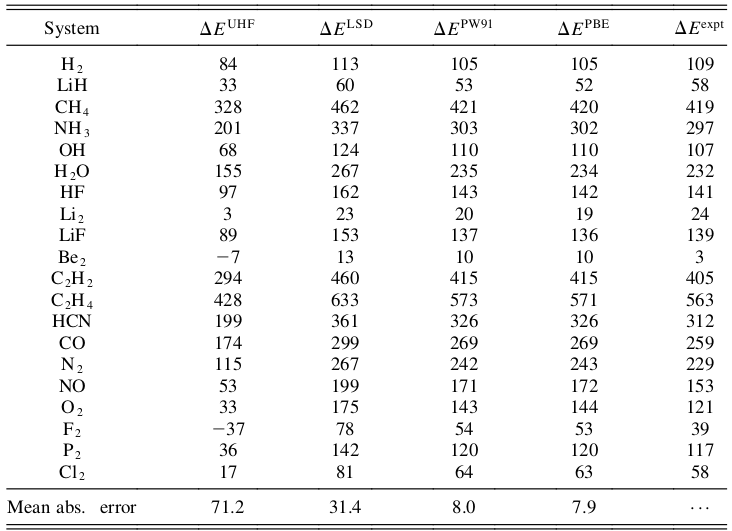
\includegraphics[scale=0.35]{Atomisation_energies_table.png}
	\end{figure}
	Taken from: \textit{GGA made simple}, John P. Perdew, Kieron Burke, Matthias Ernzerhof,Phys. Rev. Lett. 78, 1396 (1997)
	\end{frame}
	
	\begin{frame}[t]{References}
	 \begin{enumerate}
	 \item{CECAM summer school(2017) video lectures by Levy,Perdew,Kieron Burke - \\ \small\underline{\url{https://www.youtube.com/channel/UCfLssAro7SMxgaeKTNFFeeA}}}
	 \item{ABC of DFT, Kieron Burke}
	 \item{A Chemist’s Guide to
Density Functional Theory, Wolfram Koch, Max C. Holthausen}
	 \item{Electronic Structure Calculations for Solids and Molecules- Theory and Computational Methods,Jorge Kohanoff}
	 \item{GGA made simple - John P. Perdew, Kieron Burke, Matthias Ernzerhof,Phys. Rev. Lett. 78, 1396 (1997)}
	 \end{enumerate}
	\end{frame}
\end{document}